\documentclass[final]{article}
\usepackage{xcolor}
\usepackage{fontspec}
\setmainfont[
Path           = /var/www/trading_cards/fonts/,
Extension      = .otf,
Ligatures      = TeX,
BoldFont       = Dax-Bold,
ItalicFont     = Dax-Italic,
BoldItalicFont = Dax-BoldItalic,
]{Dax-Medium}

\newfontfamily\trebuchet[
Path           = /var/www/trading_cards/fonts/,
Extension      = .ttf,
Ligatures      = TeX,
]{Trebuchet MS Bold Italic}

%\newfontface\condensed{Myriad_Pro_Condensed.otf}

%\usepackage[T1]{fontenc}
%\usepackage{textcomp}
%\usepackage{MyriadPro}
%\usepackage[sfdefault]{noto}
%\renewcommand\familydefault{\sfdefault} 
%\usepackage[T1]{fontenc}



\usepackage{calc}


\usepackage{environ}% http://ctan.org/pkg/environ
%\usepackage{lipsum}% http://ctan.org/pkg/lipsum
\newdimen\fontdim
\newdimen\upperfontdim
\newdimen\lowerfontdim
\newif\ifmoreiterations
\fontdim12pt

\makeatletter
\NewEnviron{fitbox}[2]{% \begin{fitbox}{<width>}{<height>} stuff \end{fitbox}
	\def\buildbox{%
		\setbox0\vbox{\hbox{\minipage{#1}%
				\fontsize{\fontdim}{1.2\fontdim}%
				\selectfont%
				\stuff%
				\endminipage}}%
		\dimen@\ht0%
		\advance\dimen@\dp0%
	}%
	\def\stuff{\BODY}% Store environment body
	\buildbox%
	% Compute upper and lower bounds
	\ifdim\dimen@>#2
	\loop
	\fontdim.5\fontdim % Reduce font size by half
	\buildbox
	\ifdim\dimen@>#2 \repeat
	\lowerfontdim\fontdim
	\upperfontdim2\fontdim
	\fontdim1.5\fontdim
	\else
	\loop
	\fontdim2\fontdim % Double font size
	\buildbox
	\ifdim\dimen@<#2 \repeat
	\upperfontdim\fontdim
	\lowerfontdim.5\fontdim
	\fontdim.75\fontdim
	\fi
	% Now try to find the optimum size
	\loop
	\message{Bounds: \the\lowerfontdim\space
	         \the\fontdim\space \the\upperfontdim^^J}
	\buildbox
	\ifdim\dimen@>#2
	\moreiterationstrue
	\upperfontdim\fontdim
	\advance\fontdim\lowerfontdim
	\fontdim.5\fontdim
	\else
	\advance\dimen@-#2
	\ifdim\dimen@<10pt
	\lowerfontdim\fontdim
	\advance\fontdim\upperfontdim
	\fontdim.5\fontdim
	\dimen@\upperfontdim
	\advance\dimen@-\lowerfontdim
	\ifdim\dimen@<.2pt
	\moreiterationsfalse
	\else
	\moreiterationstrue
	\fi
	\else
	\moreiterationsfalse
	\fi
	\fi
	\ifmoreiterations \repeat
	\box0% Typeset content
}
\makeatother


\usepackage{graphicx,changepage}

%\usepackage[absolute, overlay,showboxes]{textpos}
\usepackage[absolute, overlay]{textpos}

\usepackage{tikz}
\usepackage[pages=all]{background}
\usepackage{pdfpages}
\usepackage[abs]{overpic}
\usepackage{pict2e}
\usepackage{rotating}
\usepackage{etoolbox}

%\newcommand{\copyrightname}{Dax Regular 5}
%\newcommand{\overlay}{02_Germany} %Refs, Hamburg
%\newcommand{\teamname}{Refs} %Refs, Hamburg
%\newcommand{\playername}{Kai Haugen Shaw}
%\newcommand{\playernumber}{79}
%\newcommand{\position}{Chaser/Keeper/Seeker}

%\newcommand{\motto}{Short text}
%\newcommand{\motto}{Long enough for two lines text}
%\newcommand{\motto}{Ebis iducient et at qui aut ent omnienis esacilib usdaerchit optaque}
%\newcommand{\motto}{Lorem ipsum dolor sit amet, consetetur sadipscing elitr, sed diam nonumy eirmod tempor invidunt ut labore et dolore magna aliquyam erat, sed diam voluptua. At vero eos et accusam et justo duo dolores et ea rebum. Stet clita kasd gubergren, no sea takimata sanctus est Lorem ipsum dolor sit amet.}
%\newcommand{\cata}{11}
%\newcommand{\catb}{12}
%\newcommand{\catc}{13}
%\newcommand{\catd}{14}
%\newcommand{\backgroundimage}{examples/test}
%\definecolor{positioncolor}{cmyk}{\vpositioncolor}
%\definecolor{namecolor}{cmyk}{\vnamecolor}
%\def\vpositioncolor{0.865, 0.452, 0, 0.505}
\definecolor{positioncolor}{cmyk}{\vpositioncolor}
\definecolor{namecolor}{cmyk}{\vnamecolor}

\usepackage[paperheight=96mm,paperwidth=66mm,top=0in,bottom=0in,right=0in,left=0in]{geometry}

%\backgroundsetup{
%	scale=1,
%	color=black,
%	opacity=1,
%	angle=0,
%	contents={%
%		\includegraphics[width=\paperwidth,height=\paperheight]{\backgroundimage}
%	}%
%}

\usetikzlibrary{fadings}
\usetikzlibrary{shapes.misc, positioning}
\usetikzlibrary{shadows.blur}
\usetikzlibrary{shapes.symbols}

\begin{document}
\raggedright
\color{white}

% Team
%\begin{textblock*}{39mm}(7.3mm,16mm)
%	\noindent \fontsize{8}{8} \color{positioncolor}\selectfont\teamname
%\end{textblock*}

\newlength{\originalhight}
\newlength{\originallength}
\newlength{\perfecthight}
\setlength{\perfecthight}{10pt}
\newlength{\maxlength}
\setlength{\maxlength}{40mm}
\settoheight{\originalhight}{\noindent \fontsize{10}{10} \selectfont{\MakeUppercase{\playername}}
		\ifdim \originallength > \maxlength
		\resizebox{\maxlength}{!}{\noindent \fontsize{10}{10} \selectfont{\MakeUppercase{\playername}}}
		\else
		\noindent \fontsize{10}{10} \selectfont{\MakeUppercase{\playername}}
		\fi}

\begin{textblock*}{40mm}(5.5mm, 8.5mm + \perfecthight - \originalhight)
	\settowidth{\originallength}{\noindent \fontsize{10}{10} \selectfont\textbf{\color{namecolor}\MakeUppercase{\playername}}}
	\ifdim \originallength > \maxlength
		\resizebox{\maxlength}{!}{\noindent \fontsize{10}{10} \selectfont\textbf{\color{namecolor}\MakeUppercase{\playername}}}
	\else
		\noindent \fontsize{10}{10} \selectfont\textbf{\color{namecolor}\MakeUppercase{\playername}}
	\fi
\end{textblock*}

% Position

\begin{textblock*}{30mm}(5.5mm,14.9mm)
	\noindent \fontsize{8}{8} \selectfont \textcolor{positioncolor}{\position}
\end{textblock*}

% CATA
\begin{textblock*}{13mm}(5.3mm,34.3mm)
	\noindent \fontsize{11}{11} \trebuchet {\cata}
\end{textblock*}
% CATB
\begin{textblock*}{11mm}(5.3mm,46mm)
	\noindent \fontsize{11}{11} \trebuchet {\catb}
\end{textblock*}
% CATC
\begin{textblock*}{10mm}(5.3mm,57.5mm)
	\noindent \fontsize{11}{11} \trebuchet {\catc}
\end{textblock*}
% CATD
\begin{textblock*}{11mm}(5.3mm,69mm)
	\noindent \fontsize{11}{11} \trebuchet {\catd}
\end{textblock*}

% Number
\begin{textblock*}{12mm}(5.3mm,84mm)
	\noindent \fontsize{18}{18} \trebuchet {\#\playernumber}
\end{textblock*}

% Spruch
\ifdefempty{\motto}{}{
\newlength{\maxhight}
\setlength{\maxhight}{7.0mm}
\newlength{\boxwidth}
\settoheight{\originalhight}{\parbox{36mm}{
	\fontsize{10}{12} \selectfont \centering \motto}}
\settowidth{\boxwidth}{\fontsize{10}{12} \selectfont \centering \motto}
\newlength{\maxboxwidth}
\setlength{\maxboxwidth}{34mm}
\begin{textblock*}{\maxboxwidth}(22mm,78mm)
	\raggedright
\ifdim \originalhight > \maxhight%
\begin{tikzpicture}[overlay]
\draw [opacity=0,
blur shadow={shadow blur steps=5,shadow blur radius=5pt,shadow blur extra rounding=8pt,shadow opacity=10,shadow xshift=-4pt,shadow yshift=0}
] (3.7,0.2) rectangle (-0.2,-1.2);
\end{tikzpicture}
\begin{fitbox}{\maxboxwidth}{\maxhight}
	\selectfont \centering \motto
\end{fitbox}

	
\else%
	\ifdim \boxwidth > \maxboxwidth%
	\begin{tikzpicture}
		\node (1) [
		blur shadow={shadow blur steps=5,shadow blur radius=5pt,shadow blur extra rounding=8pt,shadow opacity=10,shadow xshift=-4pt,shadow yshift=0}
		      ] {\parbox{\maxboxwidth}{\fontsize{10}{12} \selectfont \centering \motto}};
	\end{tikzpicture}
	\else%
	\parbox{\maxboxwidth}{\centering
	\begin{tikzpicture}
	\node (1) [
	blur shadow={shadow blur steps=5,shadow blur radius=5pt, shadow blur extra rounding=8pt,shadow opacity=10,shadow xshift=-4pt,shadow yshift=0}
	] {\fontsize{10}{12} \selectfont \motto};
	\end{tikzpicture}}
	\fi%
\fi%
\end{textblock*}
}
% Function
%\begin{textblock*}{57mm}(7.62mm,88mm)
%	\noindent \fontsize{8}{8} \selectfont\textbf{\function}
%\end{textblock*}

% Copyright
\newlength{\unturnedhight}
\settoheight{\unturnedhight}{\fontsize{5}{5} \selectfont\copyright \copyrightname}
\newlength{\lencopy}
\settowidth{\lencopy}{\fontsize{5}{5} \selectfont\copyright \copyrightname}
\ifdefempty{\copyrightname}{}{
\begin{textblock*}{800mm}(58.7mm+\unturnedhight,90mm-\lencopy)
	\begin{turn}{90}
	\noindent \fontsize{5}{5} \selectfont\copyright\ \copyrightname
	\end{turn}
\end{textblock*}
}


% Picture
\begin{tikzpicture}[remember picture, overlay]
\noindent\node[inner sep=0pt] at (4.075,-4.45) {%
	\noindent\includegraphics[height=1\paperheight]{\backgroundimage}%
};%
\end{tikzpicture}

% Background
\begin{tikzpicture}[remember picture, overlay]
\noindent\node[inner sep=0pt] at (current page.center) {%
	\noindent
\includegraphics[width=\paperwidth,height=1\paperheight]{overlays/\overlay}%
};%
\end{tikzpicture}

% Background multiply
%\begin{tikzpicture}[remember picture, overlay, blend mode=multiply]
%\noindent\node[inner sep=0pt] at (current page.center) {%
%	\noindent
\includegraphics[width=\paperwidth,height=1\paperheight]{shadow}%
%};%
%\end{tikzpicture}


% Number
%\ifdefempty{\playernumber}{
%	\begin{tikzpicture}[remember picture, overlay]
%        \noindent\node[inner sep=0pt] at (current page.center) {%
%            \noindent
\includegraphics[width=\paperwidth,height=1\paperheight]{numbers/None}%
%        };%
%        \end{tikzpicture}
%	}{
%        \begin{tikzpicture}[remember picture, overlay]
%        \noindent\node[inner sep=0pt] at (4.15,-4.4) {%
%            \noindent\includegraphics[]{numbers/\playernumber}%
%        };%
%        \end{tikzpicture}
%}

%\begin{tikzpicture}[remember picture, overlay]
%\noindent\node[inner sep=0pt] at (current page.center) {%
%	\noindent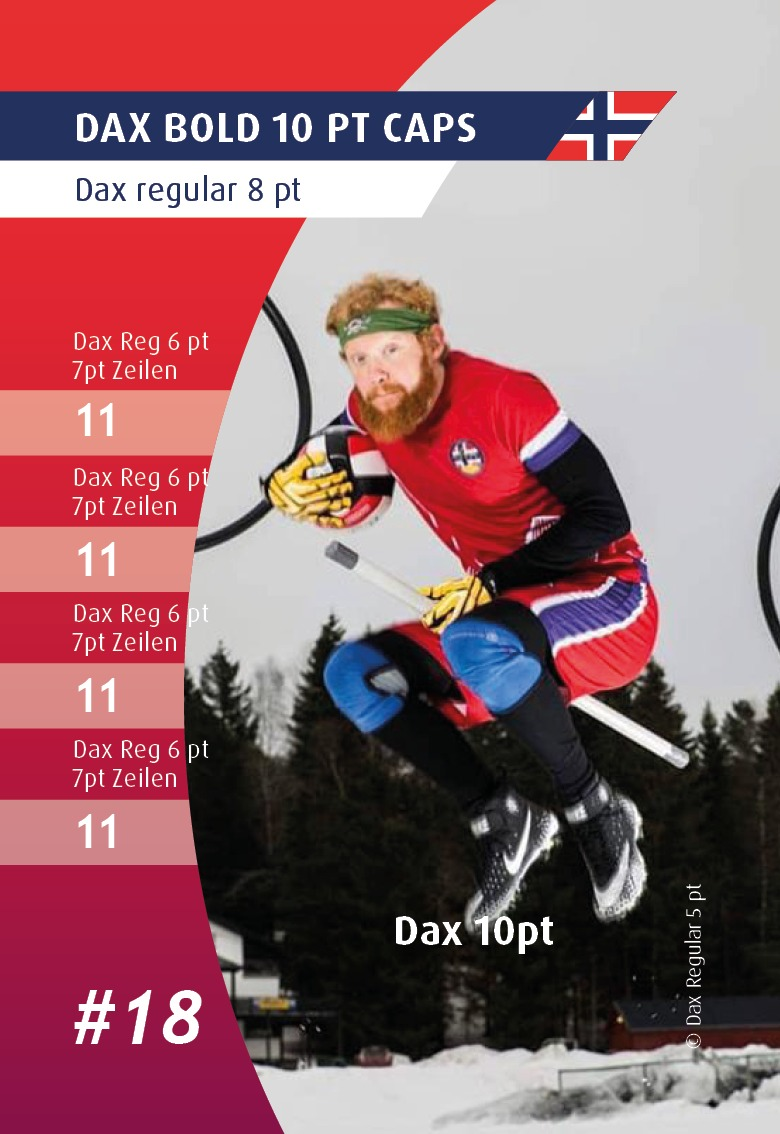
\includegraphics[width=\paperwidth,height=1\paperheight]{example}%
%};%
%\end{tikzpicture}

\end{document}
